\chapter{Conclusions}
\label{cap:conclusoes}

Chapter~\ref{cap:avaliacao} measured each component in isolation. This one brings together what
those measurements yield. It synthesises the work carried out, presents the answer obtained for
each research question, identifies the limitations of the study and sets out the lines of future
development.

\section{Main conclusions}
\label{sec:con_principais}

The work produced a system in operation and an evaluation of each of the techniques that compose
it. InvestiGator monitors twelve companies in a continuous cycle, delivers explained alerts to a
public channel and provides a page on which both the messages sent and the decisions that led to
silence are recorded. Between 9 July and 13 August 2026, $367$ messages were delivered; between
22 July and 20 August, $36{,}925$ triage decisions were logged; and the reconstruction of the
precedent base gathered $38{,}214$ cases with
measured impact. These
numbers describe a deployed system and not a demonstration built for the purpose.

The component that gives the work the character of a dissertation is not, however, the system, but
the evaluation to which it was submitted. Three of the four techniques were compared with simpler
alternatives, chosen and declared before the measurement was carried out, which is the condition
for the result to be able to be negative. In one of them the result was indeed negative. The fourth
technique, the decomposition of the movement, does not admit a comparison of the same nature, since
the split of a return has no observable external referent. What was measured of it is what remains
falsifiable: the quality of the fit that supports it, and the ability to produce distinct answers
for distinct companies.

The engineering contribution does not lie in the size of the learned model. The system trains a
single model, with nine inputs, and that model loses to a one-variable baseline. Confidence in that
value, and in the negative conclusion it supports, depends on what had to be built around it.
Section~\ref{sec:sis_ciclo} describes the seven pieces. The dataset is labelled from two
independent sources. The label is declared as a decision, and nine alternative definitions are
measured instead of the one adopted being assumed. The temporal separation is verified by an
automatic procedure. The calibration comes with the measurement and the declaration of the bias
that affects it. The artefacts are kept under version control. The deployed model is demonstrably
the model evaluated. And the system in operation continues to be observed. It is in that set, and
not in the model, that the work resides.

A second conclusion runs across the four case studies and belongs to none of them in particular.
On three distinct occasions, a simpler technique obtained a better result than a more sophisticated
one under equivalent conditions: the rolling \emph{z}-score against two learned detectors, recent
volatility against text representations, and a table of thirteen constants against the trained
model. On three other occasions the reverse happened, with the alternative measured obtaining the
better result. The system kept the deployed option for distinct reasons in each case: the equally
weighted estimator for explainability, the twenty-day window for responsiveness, and the smaller
sentence encoder for computational cost.

The distinction between these two cases is the distinction between a result and a choice, and the
present chapter keeps it explicit: what the measurement establishes is reported as a result, and
what the author decided in spite of the measurement is reported as a decision, accompanied by what
that decision costs when the measurement separates the alternatives, and by the statement that it
costs nothing in \gls{PRAUC} when it does not separate them.

\section{The answers to the research questions}
\label{sec:con_respostas}

This section answers the three questions stated in Section~\ref{sec:intro_objetivos} and
delimits, in each case, what the answer does and does not allow to be claimed.
Figure~\ref{fig:con_scorecard} brings the three together.

\begin{figure}[ht]
\centering
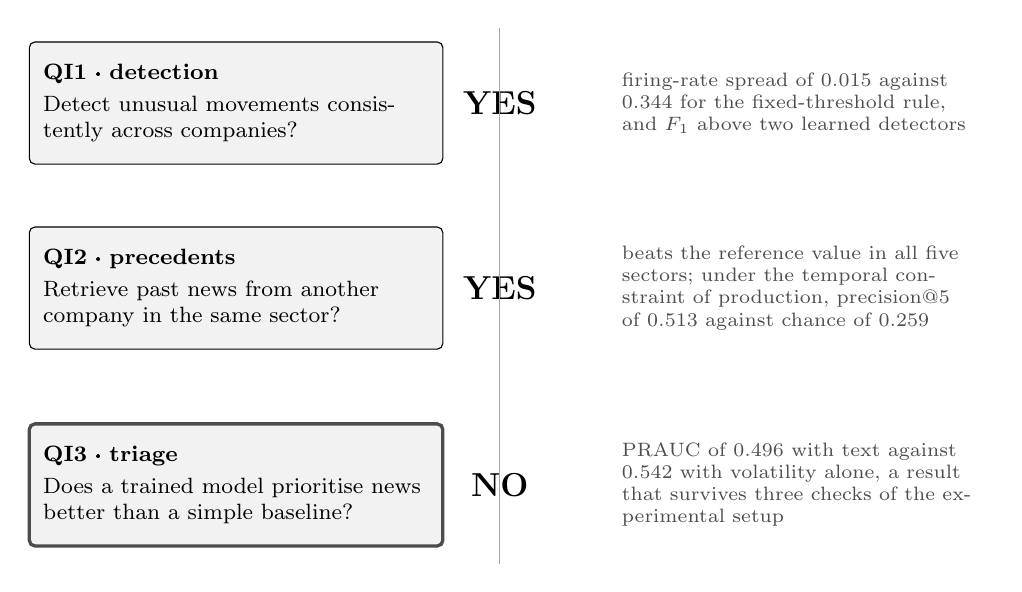
\begin{tikzpicture}[font=\footnotesize,
  cx/.style={draw, rounded corners=2pt, align=left, inner sep=5pt, text width=4.9cm,
             minimum height=1.55cm, fill=black!5},
  neg/.style={cx, draw=black!70, very thick},
  ver/.style={font=\bfseries\large, align=center},
  num/.style={align=left, text width=4.6cm, font=\scriptsize, text=black!70},
]
  \node[cx] (q1) at (0,0) {\textbf{\gls{QI}1 · detection}\\[2pt]
    Detect unusual movements consistently across companies?};
  \node[ver] at (3.35,0) {YES};
  \node[num] at (7.2,0) {firing-rate spread of $0.015$ against $0.344$ for the fixed-threshold
    rule, and $F_1$ above two learned detectors};

  \node[cx] (q2) at (0,-2.35) {\textbf{\gls{QI}2 · precedents}\\[2pt]
    Retrieve past news from another company in the same sector?};
  \node[ver] at (3.35,-2.35) {YES};
  \node[num] at (7.2,-2.35) {beats the reference value in all five sectors; under the temporal
    constraint of production, precision@5 of $0.513$ against chance of $0.259$};

  \node[neg] (q3) at (0,-4.85) {\textbf{\gls{QI}3 · triage}\\[2pt]
    Does a trained model prioritise news better than a simple baseline?};
  \node[ver] at (3.35,-4.85) {NO};
  \node[num] at (7.2,-4.85) {\gls{PRAUC} of $0.496$ with text against $0.542$ with volatility
    alone, a result that survives three checks of the experimental setup};

  \draw[black!35] (3.35,-5.85) -- (3.35,0.95);
\end{tikzpicture}
\caption[The three research questions and the answers obtained]{The three answers, with the
negative answer presented with the same prominence as the other two. The third row is the one that
gives credit to the others: a work that reports only the favourable results does not allow one to
determine whether the affirmative answers were measured or presumed.}
\label{fig:con_scorecard}
\end{figure}

\subsection{Detection of unusual movements}

The answer to \gls{QI}1 is affirmative. A \emph{z}-score over a rolling twenty-day window flags
rare days at a practically identical rate in companies of very different volatilities. The spread
between the most and the least flagged company is $0.015$, against $0.344$ for a fixed threshold
rule at three per cent. Against an approximate label, the method obtains $F_1 = 0.516$ and the
fixed rule $0.218$. Subjected to an equivalent causal protocol, the same method further beats two
detectors designed for this task, with $F_1$ of $0.530$ against $0.269$ for \emph{Isolation Forest}
\autocite{liu2008isolation} and $0.280$ for the \emph{Local Outlier Factor}
\autocite{breunig2000lof}.

The deployed configuration is not, however, the best measured within the family itself. With the
same recall, an exponentially weighted estimator obtains $F_1 = 0.664$ and a sixty-day window
obtains $0.678$, against the $0.516$ of the configuration in production. What \gls{QI}1 establishes
is that the rolling family beats the fixed threshold and the two learned detectors, and not that
the parameterisation chosen is the best of that family.

This result is less surprising than the difference in values suggests, and the literature allows
it to be situated. The two learned detectors define rarity from the geometry of the data, one by
isolating the point and the other by comparing densities, and were designed for spaces with
multiple interacting variables. The problem treated here has a single series of returns per
company, in which the relevant structure is temporal and not geometric: agitated periods follow
calm ones. It is the property that \gls{ARCH} and \gls{GARCH} models formalise
\autocite{engle1982arch, bollerslev1986garch}. The rolling window captures it directly; a detector
trained over the complete set would have to learn it. When the assumption built into a simple
method coincides with the actual structure of the problem, the margin for beating it is small.

The reach of the answer is delimited by three conditions. The comparison covers fifteen
large-capitalisation companies, selected in 2026 and evaluated over the past, which survived by
construction; three years of quotes; and a single market. The label used as a secondary argument is
itself relative to the volatility of each company, which is why the principal argument is the
consistency of the firing rate, which does not depend on labels. The three per cent threshold of
the alternative rule was not optimised, so what the comparison establishes is not that no fixed
threshold would obtain a better result, but that a fixed threshold rule measures a quantity
distinct from the one intended.

\subsection{Precedent retrieval}

The answer to \gls{QI}2 is affirmative, and its formulation requires the sector level. Over the
recent corpus, retrieval by sentence similarity \autocite{reimers2019sbert} obtains precision@5 of
$0.514$, against $0.346$ for vocabulary overlap, $0.240$ for random choice and $0.126$ for
presenting the most recent news. Here too the deployed model is not the best measured: a larger
variant obtains $0.538$ under the same protocol, and was set aside on computational cost.

The aggregate value is not, however, the appropriate way of stating the result. Almost half the
news in the corpus belongs to the technology sector, which makes available a strategy that
dispenses with any model and does not even look at the query, consisting in invariably returning
news from that sector; its precision equals the fraction of technology queries, $0.467$. That
strategy is useless as a product, since it is right on every query of one sector and on none of the
remaining four, but its existence shows that the aggregate measures in part the composition of the
corpus.

The comparison that survives the objection is carried out within each sector, where the method
beats the respective reference value in all five. The absolute margin is largest in the most
abundant sector, at $+0.283$ in technology; in the sparse sectors, where the reference value is
around $0.072$, the method obtains several times that value with a smaller absolute margin. This is
the claim the work supports.

Two further checks delimit the answer. Over the complete historical corpus, with approximately
eighty thousand news items from six years, precision rises to $0.595$. The reference value rises in
the same proportion, and the margin holds. The method does not degrade with scale, nor does it
improve with it. Imposing the constraint the system actually faces, under which the precedent must
be prior to the query, reduces precision to $0.513$ and the reference value to $0.259$, with the
margin varying by $0.008$. The method keeps its advantage when forced to operate as it operates in
production.

The second caveat has direct consequences for the product. Retrieval identifies topic and not
direction: the agreement between the direction of the movement of the query news item and that of
the precedents stands at $0.708$ against a chance value of $0.688$, a difference of $0.020$. Two
news items can deal with the same subject and the price move in opposite directions. The result is
consistent with what the semi-strong form of the efficient market hypothesis would lead one to
expect \autocite{fama1970efficient}, under which public information is already reflected in the
price, without the work testing it or relying on it to establish any conclusion. The practical
consequence is the decision to present the precedents individually, with date and outcome, rather
than summarising them into an average liable to be read as a forecast.

A final delimitation concerns the label. Membership of the same sector is a verifiable
approximation of relevance, and not the property one intended to measure. The lexical baseline is
the most elementary form of its family, without weighting by the rarity of terms and without
normalisation by length. The seventeen percentage points of advantage measure the distance to a
starting point, and not to a tuned ranking function \autocite{robertson2009bm25}.

\subsection{News triage}

The answer to \gls{QI}3 is negative. No variant incorporating the text of the headline beats a
baseline built only on the volatility of the twenty preceding days, with $0.496$ of \gls{PRAUC}
against $0.542$, and the Brier score follows the same ordering. The result survives three checks.
The first repeats the comparison granting the text the best conditions available, and raises its
best value to $0.533$, without reaching the baseline. The second resamples by groups formed by
company and day, and keeps the interval excluding zero. The third repeats the measurement for nine
alternative combinations of label threshold and horizon, and volatility matches or beats the model
with text in all nine.

The answer gained precision over the course of the work and that precision changes what is drawn
from it. The earlier comparisons place the representations side by side and therefore answer the
question of which of them is better. The question of greater use to whoever builds a system is a
different one, and consists in determining whether the text adds to what is already known. Measured
against the per-company lookup table, which contains everything the model knows about the company
and nothing about the news, the answer is affirmative: the headline adds $+0.012$ of \gls{PRAUC},
with an interval between $+0.004$ and $+0.020$, which excludes zero. It is the only occasion on
which a text representation shows a detectable increment on this task.

The value falls below the $0.02$ limit that Chapter~\ref{cap:avaliacao} fixed before the
measurements, and that limit applies in both directions. What is established is an upper bound on
the effect of the text, and not a quantity the system can make use of.

Three measurements prevent this increment from reopening the verdict. The sum does not beat
volatility alone, and the interval of the difference contains zero. The increment does not survive
the metric that describes the product: precision within the budget of five alerts per day stays at
$0.662$ with and without text. And the ability to separate news items of the same company remains
at the level of chance. What these measurements add to the negative answer is not a caveat but a
location: the information the text carries distinguishes companies and periods, when the product
needed it to distinguish news items. The formulation that survives is the weakest possible,
corresponding to an upper bound on an effect and not to a discovery.

There is an established line of research that uses text to anticipate price movements
\autocite{xing2018nlffsurvey, ding2015deep}, and this result does not contradict it. The difference
does not lie in the size of the text, since \textcite{ding2015deep} likewise operate on headlines,
but in the treatment given to it. Those authors extract event structures and train a network to
predict the direction of the movement. Here headlines are compared by similarity, and direction is
never the object of a prediction. The corpora and the evaluation horizons likewise differ. The
claim this work supports is narrower than a refutation: under this data constraint and with this
family of methods, the textual signal adds nothing to what recent volatility already indicated. The
reach of the result is therefore limited to a regime of resources and to a choice of
representation, and does not extend to language.

There is, even so, a theoretical reading that frames it and that is stated with the same caution.
The semi-strong form of the efficient market hypothesis \autocite{fama1970efficient} holds that
publicly available information is already reflected in the price. If that is so, a public headline
has, at the moment it is read, no information that recent prices do not contain, and the result
obtained is what that hypothesis would lead one to expect. The resource condition of this work
worsens the expectation rather than easing it: between the publication of a news item and its
detection by free sources a median of $353$ minutes passes, an interval during which any market
reaction has already occurred. The system observes, by construction, information that has ceased to
be new.

This reading is a framing and not a conclusion. The work does not test the efficient market
hypothesis, and a negative result obtained with one family of methods over a concrete corpus does
not confirm it; confirming it would require a design this one does not have. What the reading adds
is the reason why the result is less surprising than the initial hypothesis assumed, and why its
most likely correction lies not in the representation of the text but in the delay with which it
arrives.

\section{Objectives achieved}
\label{sec:con_objetivos}

Of the four objectives stated in Section~\ref{sec:intro_objetivos}, three are fully met and one is
met with the caveat described below.

The first objective, to build the complete system from data acquisition to the delivery of the
alert, is met. Both triggers work end to end in production, on free sources, and the path of an
event is documented in Chapter~\ref{cap:sistema} with the values of a real case.

The second objective, to evaluate each component against transparent baselines, is met for the
three techniques in which an external referent exists. In one of the cases it went beyond what was
planned: the detector was compared not only with a fixed threshold rule, but also with two learned
methods.
The decomposition of the movement is the caveat: there is no ground truth against which to measure
the accuracy of a split, so what was measured is what remains falsifiable in it, corresponding to
the quality of the fit and to the ability to discriminate. Internal comparisons that would be
possible were not carried out, such as that of the one-factor model against the two-factor model,
or that of the raw sensitivities against the shrunk ones.

The third objective, to ensure that the explanations presented are faithful to what the system
computed, is met by construction and not by subsequent verification. Every value displayed comes
from the object that computed it, and the text is composed from those pieces, so it is not possible
for the alert to state a value distinct from the one the system obtained. Faithfulness is, however,
a property of the system, and not of the relation between the system and whoever reads it; the
usefulness of the explanations for a retail investor was not measured, and
Section~\ref{sec:con_limitacoes} deals with that absence.

The fourth objective, to report the results obtained including those that do not confirm the
initial expectations, is met. The negative answer to \gls{QI}3 appears in
Figure~\ref{fig:con_scorecard} and in the body of this chapter with the same prominence as the
others, accompanied by the three checks to which it was submitted and by the three occasions on
which a simpler technique beat a more sophisticated one.

\section{Limitations}
\label{sec:con_limitacoes}

This section lists the limitations of the work in order of importance.
Table~\ref{tab:con_limites} presents them together, with the work that would close each one and the
nature of its cost; the text that follows develops the four of greatest consequence and summarises
the rest. Most are quantified. Two are not, by their nature: the absence of a controlled study is an
absence and not a measure, and the distance between each label and the property it approximates
would only be measurable against a human annotation that does not exist.

\begin{table}[!htbp]
\caption[The limitations and the work that would close them]{The eleven limitations, in order of
importance, with the work that would close each one and the nature of the cost of that work. The
two that depend on calendar time are the ones that require human judgement, and they are also the
two on which the rest most depend: until a sample annotated by people exists, neither the
usefulness of the explanations nor the quality of the labels ceases to be an approximation.}
\label{tab:con_limites}
\centering
\footnotesize
\begin{tabular}{@{}L{0.33\textwidth} L{0.32\textwidth} L{0.20\textwidth}@{}}
\toprule
\tabhead{Limitation} & \tabhead{What closes it} & \tabhead{Cost} \\
\midrule
No controlled study with people & Run the protocol designed, with six to ten participants &
calendar time \\
The score is almost constant within each company & Inputs that vary from one headline to the next &
small \\
The label may favour the winning baseline & Rebuild the target with estimated sensitivities &
small \\
The labels are verifiable approximations & Annotate a sample with human judgement &
calendar time \\
The alert claims more evidence than it has & Measure impact per news item and not per day &
intraday data \\
The three blocks barely share companies & A split of constant composition & small \\
Only the headline is read, not the body of the article & Collect and represent the full text &
new data \\
The split is not always well estimated & Display the fit alongside each split & small \\
Drift is measured and not corrected & Retrain with the production log & small \\
Source coverage is incomplete and uneven & Add sources, or declare the limit &
outside our control \\
The three causes of the delay are not separated & Log when each item appears in the feed &
instrumentation \\
\bottomrule
\end{tabular}
\end{table}

\paragraph{No controlled study with users was carried out.}
This is the gap of greatest weight. The system rests on the hypothesis that an explanation
accompanied by its evidence leads a non-specialist to a better decision, and that hypothesis was not
submitted to an experimental design. The protocol exists, with participants, tasks and criteria
defined, and was not executed. What does exist, and is reported in Section~\ref{sec:av_feedback}, is
feedback collected in a real context: readers of the public channel rate the alerts they receive,
under analysis rules fixed before the first vote, and the collection continues. The literature is
explicit about the weight of this absence: claims of interpretability demand evaluation and are not
established by declaration \autocite{doshivelez2018considerations}. The reason is not a formal one.
The effect of an explanation on a person is not deducible from its construction: it is known that
trust in automated systems fails in both directions, with the user ignoring a correct warning or
accepting an incorrect one \autocite{lee2004trust}, and that the mere presence of an explanation
increases the acceptance of wrong answers \autocite{bansal2021whole}. The system was built to
produce appropriate trust, presenting evidence rather than issuing a verdict, but that it succeeds
remains a hypothesis. In the absence of the study, the two failure modes are indistinguishable in
the logs: an ignored alert and an unduly believed alert produce the same absence of data.

The distinction between the two determines what each one allows to be claimed. The channel
feedback is observational: whoever wants to votes, which shifts the sample towards the extremes; no
group received the price change without the explanation that accompanies it, so nothing attributes
the usefulness to the explanation itself; and the channel is public, so it is not known whether
those who answer belong to the audience this work assumes. What those votes measure is perceived
usefulness among those who chose to answer. The founding hypothesis concerns a better decision,
which is another quantity, and it is that one which remains untested.

\paragraph{The deployed model could not perform the function assigned to it.}
The variant put into production as a decision gate receives seven company-level inputs, one
day-level input and a single one that varies from one headline to the next, the length of the
headline. Its score is, by arithmetic and not by accident, almost constant within each company: the
mean spread within each company is $0.072$ and the spread between the medians of the companies is
$0.392$. In $48\%$ of the distinct headlines, the outcome was determined before the headline was
read.

Two claims must be separated, since only one of them is an error. The result of \gls{QI}3 stands,
because the variant with text had three hundred and eighty-four numbers per headline and still
lost. The product decision was wrong, and the reason is methodological: the choice was made by a
metric that interrogates the ordering of the complete set, when the product needed the distinction
between two headlines of the same company.

The system was changed and the model ceased to be a gate and became a ranking criterion. That
change is not validated. Over the $825$ decisions matured in production, grouped into the $239$
independent units the label admits, the ranking ability is $0.486$, with an interval between $0.403$
and $0.571$, which contains chance. Ranking is the least indefensible use of the model, and not a
demonstrated use.

This failure belongs to a class described in the literature on machine learning systems in
production. \textcite{sculley2015debt} identify a cost that appears in no quality metric, and that
comes from data dependencies and from entanglement between components: the validity of one piece
depends on assumptions about another that were never stated. The model was evaluated in isolation,
over the distribution of the training set, and deployed behind two filters that alter it. No test
failed and no log flagged an anomaly. A learned component is evaluated where it is trained and is
useful where it is placed, and when those two places differ the difference does not announce
itself.

\paragraph{The label may favour the winning baseline.}
The label discounts the movement of the market assuming unit sensitivity, so its error is not
random: it is larger in the stocks most sensitive to the market, which are typically the most
volatile. The winning baseline is precisely volatility. With what is measured it is not possible to
separate the hypothesis that volatility better predicts materiality from the hypothesis that
volatility better predicts the error of the label. Both the level and the ordering of the
\gls{QI}3 metrics are therefore conditional on the label used.

\paragraph{The alert claims more evidence than it has.}
When it displays three precedents that agree on the direction of the movement, the alert presents
that agreement as resulting from three observations. The impact is, however, measured per pair
formed by company and day, so three headlines of the same company on the same day share the value
by construction. Over the $247$ alerts with precedents delivered, in $36.8\%$ the cases displayed
rest on fewer distinct days than the number of cases presented, and in $11.3\%$ they all
correspond to the same
day; of the $120$ alerts that claim unanimity, $23.3\%$ rest on a single day. The wording of the
text was corrected to count days and not headlines, which makes the claim true. The cause remains:
while impact is measured per day, two news items of the same day are not two independent
observations.

\paragraph{The remaining seven, in summary.}
The \textbf{labels are approximations}: relevance is approximated by membership of the same sector,
materiality by the occurrence of a movement above a threshold, and rarity by a percentile of the
company's own returns. All three are objective and verifiable, and none corresponds exactly to the
property one intended to measure. Dependence on approximations is not peculiar to this work: in
neighbouring financial domains, such as fraud detection, unsupervised methods occupy a central
position because labelled anomalies are scarce \autocite{ahmed2016financial}.

The \textbf{three data blocks barely share companies}. The training block contains thirteen
companies and the test block nine, five companies from training do not appear once in the test, and
one company accounting for $17.1\%$ of the test rows never appears in training. The finding acts in
both directions: it reinforces the negative result, because a model whose signal is essentially the
identity of the company estimates it over a set almost absent from the block where it is evaluated;
and it limits it, because it does not allow the hypothesis that the model is worse to be separated
from the hypothesis that identity does not transfer between these two periods.

The \textbf{news is read only at headline level}. The system represents the headline and not the
body of the article, which limits what the text representation can capture and is a plausible,
though unconfirmed, explanation for the negative result of \gls{QI}3. Reviews of textual analysis in
finance describe works that operate over complete documents \autocite{kearney2014textual}, and a
headline is the part of the document where the most information has been discarded.

The \textbf{split of a movement is not always well estimated}. The sum of the three parts holds by
construction and validates nothing. The informative measure is the coefficient of determination in
the estimation window, whose median was $0.460$ and which in one of the seventeen companies took a
negative value; in those cases the split continues to be displayed and should be read as
indicative. Precision-weighted shrinkage \autocite{vasicek1973beta} limits the damage of a bad
estimate without turning it into a good one.

\textbf{Drift is measured and not corrected}. The parameters were estimated between 2018 and 2023
and were not readjusted. Between the training block and the test block, the population stability
index places twenty-day volatility in the band of significant displacement, at $0.281$, and that is
the input on which the model most depends. The concept drift literature deals with this problem,
with a taxonomy of the change and strategies for detection and adaptation
\autocite{gama2014survey}; here detection exists and adaptation does not. The architecture that
would supply it is defined in Section~\ref{sec:sis_ciclo}, with a conditional trigger, a rolling
window and a promotion gate, and was not executed: the limitation is one of execution and not of
design.

\textbf{Source coverage is incomplete and uneven}. There was at least one relevant news item on
$88.5\%$ of the $417$ days the detector considered unusual, and the worst covered company stands at
$50\%$. On the remaining days no change to the system has any effect, since a news item not
associated with the company by the source never enters the path. The value is an upper bound: it
establishes that a news item existed, and not that the appropriate news item arrived.

The \textbf{delay is in discovery, and its three causes are not separated}. Over the $278$ alerts
with a publication time and a send time, the median between publication and detection is $353$
minutes, and the median between detection and delivery is $5$ seconds. The move from a best-effort
scheduler to a sixty-second cycle did not reduce the delay, which rules out the polling cadence as
the explanation. Three causes remain that the history does not separate, and only one of them, the
source listing late, would be mitigated by a paid service; the other two persist with any
source.

\section{Future work}
\label{sec:con_futuro}

The lines stated in this section derive from the limitations of the previous section, according to
the correspondence presented in Table~\ref{tab:con_limites}, and are ordered by the relation
between expected effect and cost. A list of future work that does not derive from measured
limitations is a justification in another form. Figure~\ref{fig:con_futuro} groups them by what
each one requires before it can be carried out.

\begin{enumerate}
  \item \textbf{Run the study with users.} Six to ten participants, with sessions of approximately
        fifteen minutes, comparing the reading of an isolated fact with the reading of the complete
        alert. It closes the central claim of the work, which is that the evidence presented
        alongside the alert leads to a better decision. It shares with the construction of an
        annotated target, the third item of this list, the property that no computational means
        accelerates it, since both depend on human judgement. Other claims remain to be verified
        independently of it, among them the quality of the three labels, the usefulness of the
        model over the population it actually observes and the stability of the result across
        periods.
  \item \textbf{Give the decision model inputs that vary with the news.} It is the direct
        correction of the limitation of greatest technical consequence, and its cost is small, since
        the two most obvious quantities are already computed by the system: the similarity of the
        best precedent retrieved and the direction agreement among the precedents. Unlike volatility
        and sector, both vary from one headline to the next.

  \item \textbf{Build a target with human judgement.} Annotating a sample of days, identifying
        which of the news items suppressed today should pass and which of those that pass add
        nothing, would supply for the first time a real target to optimise, in place of tuning
        constants against an approximation. The same sample would allow the quality of the three
        labels used to be estimated.

  \item \textbf{Rebuild the label with estimated sensitivities.} The triage label discounts the
        movement of the market assuming unit sensitivity, which introduces an error correlated with
        the volatility of the company, which is precisely the winning baseline. Redoing the target
        with the shrunk sensitivities described in Section~\ref{sec:met_decomposicao} and repeating
        the six families of models would determine whether the ordering obtained survives an
        alternative definition of materiality.

  \item \textbf{Read the body of the articles and not only the headline.} It is the most direct
        hypothesis for explaining the negative result of \gls{QI}3 and is testable with the protocol
        already built, requiring only the collection of the full text.

  \item \textbf{Detect repeated stories by meaning.} Suppression of repetitions rests today on
        vocabulary overlap, and doing it by similarity would use the technique the system already
        has. The point matters more than its technical size suggests: if the retail investor buys
        the assets that capture their attention \autocite{barber2008glitters}, a system that
        communicates the same story three times is not informing, but amplifying the same
        stimulus.

  \item \textbf{Remove the asymmetry of reference in the same-day return.} The input corresponds,
        in training, to the complete movement of the day of the news, and in production to the last
        bar available at the moment of scoring. Replacing it with the return accumulated up to
        publication, or, more conservatively, with the previous day's return, removes the difference
        and allows performance to be reported under a single reference. The direction of the effect
        is known and favours the negative result, so the correction would reinforce it rather than
        undo it; what the experiment adds is the measurement of that reinforcement instead of its
        deduction.

  \item \textbf{Group the precedents by company-day pair before selection.} The correction applied
        to the text of the alert made the claim true without removing the cause. Selecting the
        candidates after grouping by day, displaying from each day only the closest headline,
        eliminates at source the possibility of one day observed three times being presented as
        three agreeing cases.

  \item \textbf{Expose the quality of the fit in the message itself.} The split of a movement is
        displayed with the same confidence when the coefficient of determination of the window is
        high and when it is negative. Presenting it alongside the split, and adding an explicit note
        below a minimum threshold, turns a limitation declared today only in the document into a
        property observable by whoever reads the alert.

  \item \textbf{Retrain the model with the production log.} Drift is measured and the new labels
        derive from prices, so execution is possible. The impediment is not technical, since a
        retraining would change the values reported in this document and would require evaluation
        time of its own.
\end{enumerate}

\begin{figure}[ht]
\centering
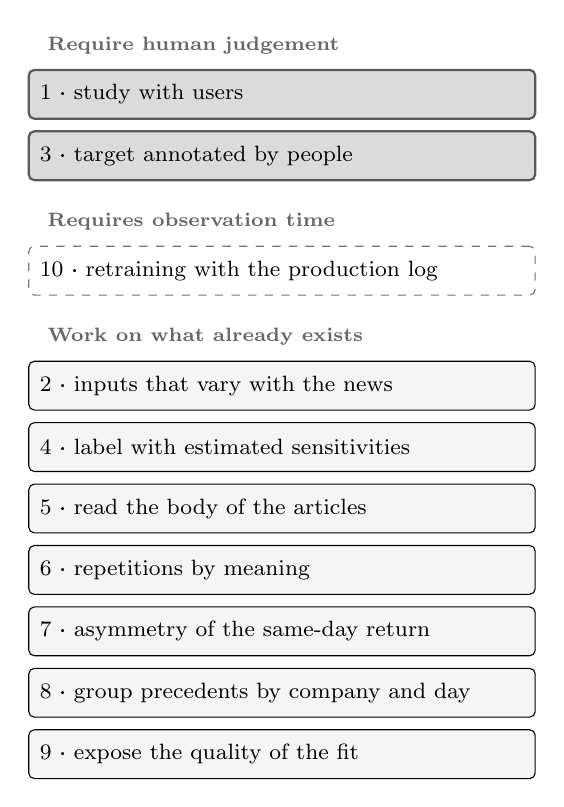
\begin{tikzpicture}[font=\footnotesize,
  it/.style={draw, rounded corners=2pt, align=left, inner sep=4pt, text width=6.15cm,
             minimum height=0.62cm, fill=black!4},
  hum/.style={it, fill=black!14, draw=black!65, thick},
  obs/.style={it, fill=white, draw=black!55, dashed},
  rot/.style={font=\scriptsize\bfseries, text=black!60, anchor=west},
]
  \node[rot] at (0,0.62) {Require human judgement};
  \node[hum] (a) at (3.1,0)     {1 · study with users};
  \node[hum] (b) at (3.1,-0.78) {3 · target annotated by people};

  \node[rot] at (0,-1.62) {Requires observation time};
  \node[obs] (c) at (3.1,-2.24) {10 · retraining with the production log};

  \node[rot] at (0,-3.08) {Work on what already exists};
  \node[it] (d) at (3.1,-3.70) {2 · inputs that vary with the news};
  \node[it] (e) at (3.1,-4.48) {4 · label with estimated sensitivities};
  \node[it] (f) at (3.1,-5.26) {5 · read the body of the articles};
  \node[it] (g) at (3.1,-6.04) {6 · repetitions by meaning};
  \node[it] (h) at (3.1,-6.82) {7 · asymmetry of the same-day return};
  \node[it] (i) at (3.1,-7.60) {8 · group precedents by company and day};
  \node[it] (j) at (3.1,-8.38) {9 · expose the quality of the fit};
\end{tikzpicture}
\caption[The future lines, by what unblocks them]{The ten lines of future work, grouped by what
each one requires before it can be carried out. Seven operate on components the system already has
and depend only on technical work. One awaits observation time, which began to run in September
2026. Two require human judgement and are the only ones that no computational means accelerates,
which places them on the critical path despite not being the ones of greatest technical cost. The
numbering is that of the list in this section, which is ordered by the relation between expected
effect and cost.}
\label{fig:con_futuro}
\end{figure}

One path was considered and not followed, and the reasons are recorded because they are needed by
whoever takes up the work. Conformal prediction allows sets of answers to be returned with a
distribution-free guarantee \autocite{vovk2005algorithmic, angelopoulos2023conformal}, which suits
a tool that refuses to claim more than it knows. Two reasons ruled it out. The first is that the
guarantee is marginal, holding on average over cases and not case by case, which is precisely the
reading a non-specialist user would make.

The second is more decisive: the guarantee requires exchangeability between calibration and test,
and these data are a time series, in which the headlines arrive in order. It is the same assumption
this work refuses when it splits the set by date and with an embargo. Applying the method without
addressing that point would produce intervals with a guarantee the data do not support, replacing
an honest value with a value that has the appearance of rigour.

\section{Final considerations}
\label{sec:con_final}

The work started from three questions a retail investor asks when faced with a price movement, and
which free tools do not answer. Whether the movement is unusual. Whether the origin is the company
or the market. And whether precedents with a known outcome exist. A system was built that answers
all three with verifiable evidence and without issuing forecasts, and each component was evaluated
against simpler alternatives declared before the measurement.

The result with the greatest informative value is negative. The hypothesis that the text of the
news would carry information absent from the prices was not confirmed over this corpus.
Investigating it produced a diagnosis of wider reach than the question that gave rise to it. The
learned component was evaluated over one distribution and deployed over another, and the metric by
which it was selected posed a question distinct from the one the product needed. No automatic test
flagged the discrepancy, because each component fulfilled its contract and what was wrong was an
assumption about the link between them.

The founding constraint of the work, under which the system produces no price forecasts, proved to
be the decision of widest reach. It determines what can be claimed: every claim of the system is
confirmable against the record at the moment it is read. It determines the form of the explanation,
which presents individual cases instead of averages. And it determines the evaluation criterion,
which bears on the ability to identify what is unusual and not on the ability to anticipate. A
system that presents evidence instead of verdicts delivers less than a system that announces
directions, and delivers only what it can support.

\begin{figure}[!htbp]
\centering
\begin{tikzpicture}[font=\footnotesize,
  est/.style={draw, rounded corners=2pt, align=left, inner sep=3pt, text width=5.1cm,
              minimum height=0.95cm, fill=black!6},
  abe/.style={draw, dashed, rounded corners=2pt, align=left, inner sep=3pt, text width=5.1cm,
              minimum height=0.95cm, fill=white, draw=black!65, thick},
  cab/.style={font=\scriptsize\bfseries, text=black!65},
  >={Stealth[length=2.2mm]},
]
  \node[cab] at (0,0.82) {WHAT IS ESTABLISHED};
  \node[est] (a) at (0,0.10)  {every quantity comes from the component that computed it};
  \node[est] (b) at (0,-0.95) {it can be checked against the record when it is read};
  \node[est] (c) at (0,-2.00) {the policy that decides the silence is documented and measured};

  \node[cab] at (6.9,0.82) {WHAT IS NOT};
  \node[abe] (d) at (6.9,-0.25) {that this explanation leads to a
    \textbf{better decision}};
  \node[align=left, text width=5.1cm, font=\scriptsize, text=black!62] (e) at (6.9,-1.75)
    {It is the founding hypothesis of the work. It remains untested, and its test is the
     first line of future work.};
  \draw[->, black!50] (d) -- (e);
  \draw[black!25] (3.45,1.0) -- (3.45,-2.5);
\end{tikzpicture}
\caption[The boundary of what the work establishes]{The exact limit of the claim. On the left, the
three properties the system demonstrates and that are verified by inspecting what it produces. On
the right, the proposition the work did not test: that presenting the evidence alongside the alert
leads to a better decision. The separation is not a courtesy caveat, since the second is the
hypothesis that motivated the work, and distinguishing it from what was demonstrated is what
prevents the first from being read as though the second were proved.}
\label{fig:con_fronteira}
\end{figure}

The contribution is therefore stated at its exact level. What this work establishes is that the
system is technically prepared to support explanations resting on verifiable historical evidence:
every quantity presented comes from the component that computed it, can be checked against the
record at the moment it is read, and the policy that decides the silence is documented and
measured. What this work does not establish is that this form of explanation leads the retail
investor to a better decision. That is the founding hypothesis, it remains untested, and its test
is the first item of the previous section. Figure~\ref{fig:con_fronteira} presents the
separation.
